\documentclass[sigconf,nonacm]{acmart}

\usepackage{booktabs}
\usepackage{multirow}
\usepackage{tabularx}
\usepackage{tikz}
\usetikzlibrary{arrows.meta,positioning,fit}

\setcopyright{none}
\settopmatter{printfolios=true}
\renewcommand\footnotetextcopyrightpermission[1]{}
\pagestyle{plain}

\title{VibeGuard: Oracle-Guided Detection and Repair of Security Weaknesses in LLM-Generated Python}

\author{Haylemicheal Mekonnen}
\affiliation{%
  \institution{Paris Lodron University of Salzburg}
  \city{Salzburg}
  \country{Austria}}

\author{Eslam Younis}
\affiliation{%
  \institution{Paris Lodron University of Salzburg}
  \city{Salzburg}
  \country{Austria}}

\author{Elbetel Reta}
\affiliation{%
  \institution{Paris Lodron University of Salzburg}
  \city{Salzburg}
  \country{Austria}}

\begin{abstract}
Large language models (LLMs) can generate functionally plausible code while
silently violating security requirements. We present VibeGuard, a layered
Python analysis and repair system that combines 40 AST security rules, a
lightweight taint extension, ten execution-based probes, exploitability
scoring, and deterministic and LLM-based repair. We evaluate VibeGuard on 500
independent solutions generated by four immutable OpenAI model snapshots for
25 CWEval tasks, together with 25 secure human references. On the 504 samples
with definitive behavioral oracles on our platform, functional pass rates are
91.7--95.8\%, but only 62.5--70.8\% of generated programs are both functional
and secure. Thus, 20.8--32.5\% are functional yet insecure. For exact
target-CWE prediction, VibeGuard obtains F1=0.664, compared with 0.230 for
Semgrep and 0.039 for Bandit; paired differences are statistically significant.
VibeGuard also achieves the highest alert and target-recall rates on SALLM and
SecurityEval. Conservative dynamic confirmation eliminates false positives in
our observed sample, but confirms only 7.6\% of all insecure cases. LLM repair
restores both functionality and security for 77 of 86 eligible samples
(89.5\%), versus 19 (22.1\%) for deterministic repair, while also causing 38
secure-to-insecure regressions outside the eligible subset. The results show
that static detection, behavioral oracles, and post-repair validation are
complementary rather than interchangeable.
\end{abstract}

\keywords{large language models, secure code generation, static analysis,
dynamic analysis, automated program repair, CWEval}

\begin{document}
\maketitle

\section{Introduction}

LLM-based coding assistants have made code generation a routine development
activity. Functional benchmarks such as HumanEval measure whether generated
programs satisfy examples and unit tests, but they do not establish that a
functionally correct implementation is secure. Prior studies of code
assistants found frequent security weaknesses in generated suggestions
\cite{pearce2022asleep,perry2022users}. Security-oriented benchmarks therefore
need to distinguish at least four outcomes: incorrect and insecure, incorrect
but secure, correct but insecure, and correct and secure.

CWEval provides that distinction through paired functional and security
oracles for security-critical programming tasks \cite{peng2025cweval}. Its
outcome-driven design also exposes a limitation of conventional static
evaluation. A static analyzer can flag a risky syntax without proving
exploitability, miss a semantically equivalent vulnerability, or report a
target CWE in code that nevertheless satisfies the security oracle. Conversely,
a generated implementation can avoid a target pattern while still violating
the intended security property. Static alerts and behavioral outcomes are
therefore related measurements, not substitutes.

We develop \emph{VibeGuard}, a research-oriented analyzer for Python code. It
combines AST pattern rules, a small taint analysis, isolated adversarial probes,
risk scoring, and two repair strategies. More importantly, its evaluation
pipeline preserves model responses and metadata, runs independent behavioral
oracles, compares three analyzers in normalized CWE space, and uses repeated
samples per task rather than pooling unrelated tasks for pass@k estimates.

This paper answers six research questions:

\begin{description}
  \item[RQ1:] How often do current models produce functional, secure, and
  functional-but-insecure solutions?
  \item[RQ2:] How accurately does VibeGuard detect behavioral insecurity
  compared with Bandit and Semgrep?
  \item[RQ3:] How does security change when developers can inspect up to five
  independent generations for the same task?
  \item[RQ4:] What precision--recall trade-off is introduced by dynamic
  confirmation and exploitability scoring?
  \item[RQ5:] Can deterministic or LLM repair restore behavioral security
  without breaking functionality?
  \item[RQ6:] Do the detection results generalize to SALLM, SecurityEval, and
  benign algorithmic references from EvalPlus?
\end{description}

Our main contributions are:
\begin{itemize}
  \item a layered analyzer with 40 security rules, ten adversarial probes, and
  repair acceptance gates that reject newly introduced finding types;
  \item a reproducible corpus of 500 generated solutions from four pinned model
  snapshots, with five independent samples for each model--task pair;
  \item an oracle-centered evaluation using exact-CWE metrics, task-clustered
  confidence intervals, paired significance tests, and secure@k estimates; and
  \item an empirical characterization of both repair success and repair harm,
  including semantic regressions that static post-checks fail to detect.
\end{itemize}

\section{Background and Related Work}

\subsection{Evaluating Generated Code}

HumanEval popularized pass@k for code generation \cite{chen2021codex}. EvalPlus
later showed that limited tests can substantially overestimate functional
correctness and even mis-rank models \cite{liu2023evalplus}. CWEval extends the
outcome-driven approach to security: each task has a precise specification, a
secure reference, and separate functional and security tests
\cite{peng2025cweval}. This design is central to our study because it permits an
independent label for security instead of treating an analyzer's own output as
ground truth.

SALLM introduced a security-centric prompt collection and security-aware
variants of pass@k \cite{siddiq2024sallm}. SecurityEval provides 121 labeled
Python vulnerability examples mined from public security documentation
\cite{siddiq2022securityeval}. These datasets broaden CWE coverage, but each
record supplies only one intended positive CWE label. Consequently, a second
correct alert in the same program cannot be identified as a false positive
without full multi-label annotation. We therefore report target recall and
overall alert incidence on these datasets, rather than claiming precision.

\subsection{Security of LLM-Generated Code}

Pearce et al. found vulnerable Copilot suggestions across multiple CWE
scenarios \cite{pearce2022asleep}; user studies further indicate that access to
an AI assistant can increase the production of insecure code and user
confidence in that code \cite{perry2022users}. Work such as SVEN and SafeCoder
changes model behavior through security-specific fine-tuning
\cite{he2023sven,he2024safecoder}. Our work instead studies a post-generation
control: analyze an arbitrary generated program, optionally confirm a finding,
then repair and re-evaluate it against an external oracle.

\subsection{Detection and Repair}

Bandit is an AST security linter specialized for Python \cite{bandit}; Semgrep
matches declarative patterns and supports community security rules
\cite{semgrep}. Both are useful baselines, but neither baseline is optimized for
the exact behavioral contracts in CWEval. LLMs have also shown strong potential
for program repair \cite{xia2023repair}. However, a reduced static finding count
does not prove semantic preservation. We therefore count a repair as successful
only when the original program is functional and insecure and the repaired
program passes both oracle classes.

\section{VibeGuard}

Figure~\ref{fig:architecture} summarizes the system. The layers are separated
so that detection never depends on repair, and static analysis does not execute
the subject program.

\begin{figure*}[t]
\centering
\resizebox{0.98\textwidth}{!}{%
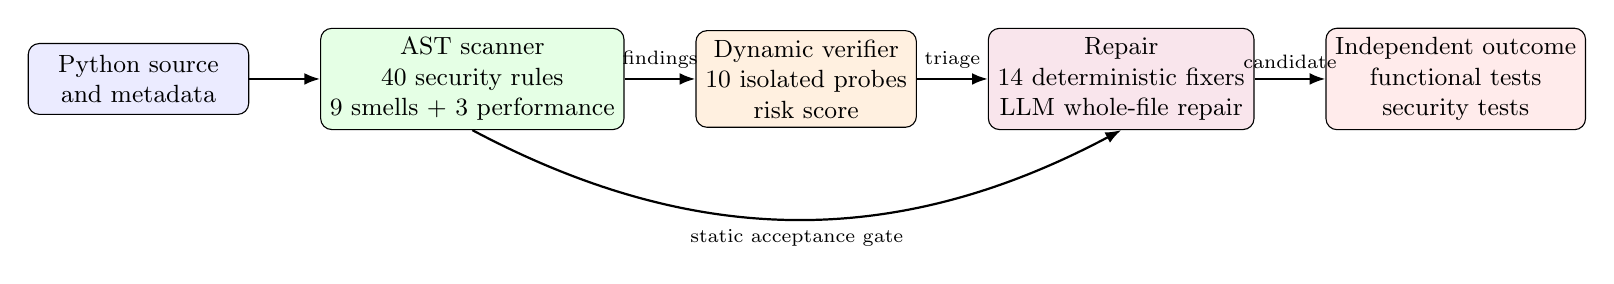
\begin{tikzpicture}[
  node distance=7mm and 9mm,
  box/.style={draw, rounded corners, align=center, minimum height=9mm,
              minimum width=28mm, font=\small},
  arrow/.style={-{Latex[length=2mm]}, thick}
]
\node[box, fill=blue!8] (input) {Python source\\and metadata};
\node[box, fill=green!10, right=of input] (scan) {AST scanner\\40 security rules\\9 smells + 3 performance};
\node[box, fill=orange!12, right=of scan] (probe) {Dynamic verifier\\10 isolated probes\\risk score};
\node[box, fill=purple!10, right=of probe] (repair) {Repair\\14 deterministic fixers\\LLM whole-file repair};
\node[box, fill=red!8, right=of repair] (oracle) {Independent outcome\\functional tests\\security tests};
\draw[arrow] (input) -- (scan);
\draw[arrow] (scan) -- node[above,font=\scriptsize]{findings} (probe);
\draw[arrow] (probe) -- node[above,font=\scriptsize]{triage} (repair);
\draw[arrow] (repair) -- node[above,font=\scriptsize]{candidate} (oracle);
\draw[arrow, bend right=28] (scan.south) to node[below,font=\scriptsize]{static acceptance gate} (repair.south);
\end{tikzpicture}
}
\caption{VibeGuard's evaluation path. Static analysis, dynamic confirmation,
repair, and behavioral oracles provide distinct evidence.}
\Description{A left-to-right architecture from Python source through static
scanning, dynamic probes, repair, and independent functional and security
oracles.}
\label{fig:architecture}
\end{figure*}

\subsection{Static Analysis}

The scanner parses source with Python's \texttt{ast} module and applies 40
security rules. The rule set covers injection, unsafe execution,
deserialization, path handling, cryptography, transport security, web output,
authentication state, temporary files, privileges, and sensitive data. Each
finding records a rule identifier, severity, category, CWE, source location,
and remediation suggestion. Nine maintainability rules and three performance
rules run in the same scanner but remain separate categories.

Table~\ref{tab:rule-coverage} groups the security rules by the behavior they
approximate. The categories are organizational rather than mutually exclusive:
for example, unsafe deserialization is both an injection primitive and a data
integrity failure. Rules operate on AST nodes rather than source-string regular
expressions. They resolve imported and qualified call names where possible,
inspect keyword arguments, and attach metadata only after a rule emits a
finding. This separation keeps syntactic matching independent from severity,
CWE, and OWASP labels and lets the experiment normalize findings without using
free-form messages.

\begin{table*}[t]
\caption{Coverage of the 40 VibeGuard security rules. Probe counts refer to
execution-based confirmations; all other rules remain static-only.}
\label{tab:rule-coverage}
\centering
\small
\begin{tabularx}{\textwidth}{lrrXl}
\toprule
Rule family & Rules & Probes & Representative behaviors & Representative CWEs \\
\midrule
Code, command, and data injection & 9 & 3 & \texttt{eval}/\texttt{exec}, shell execution, SQL construction, pickle/YAML loading, XPath and XML construction & 78, 89, 91, 95, 502, 643 \\
Web request and output handling & 7 & 4 & SSRF, HTML output, redirects, URL allow-lists, log and HTTP-header injection, output encoding & 20, 79, 113, 116, 117, 601, 918 \\
Cryptography, identity, and secrets & 10 & 1 & hard-coded secrets, weak randomness and hashing, TLS verification, weak keys, cookies, plaintext credentials, JWT verification & 295, 312, 326, 327, 329, 338, 347, 522, 614, 798 \\
File and operating-system boundaries & 6 & 1 & path traversal, XXE, temporary files, privileges, upload validation, and file permissions & 22, 250, 377, 434, 611, 732 \\
Validation and availability & 7 & 1 & assertions as validation, debug mode, generic input checks, ReDoS, CSRF, null dereference, divide-by-zero & 20, 352, 369, 400, 476, 489, 617 \\
Sensitive logging & 1 & 0 & logging password, token, credential, or secret-bearing values & 200 \\
\midrule
Total & 40 & 10 & & \\
\bottomrule
\end{tabularx}
\end{table*}

Two rules, server-side request forgery and unsafe HTML output, can invoke a
lightweight taint tracer. The tracer follows parameters through assignments and
simple expression chains to recognized sinks. It is intentionally
intra-procedural and conservative; it is not a substitute for a whole-program
data-flow engine.

The remaining 12 checks are retained because generated code can be functional
and secure while still being difficult to review or needlessly expensive.
They are never included in detector precision or recall. Category separation
is also enforced in repair: a candidate is checked against the multiplicity of
each category--rule pair, so a smell cannot be misreported as a security
success.

\subsection{Dynamic Confirmation and Risk}

Ten security rules have execution-based probes: SQL injection, path traversal,
command injection, unsafe deserialization, regular-expression denial of
service, URL validation bypass, unsafe HTML output, HTTP header injection, log
injection, and weak asymmetric keys. A probe creates an isolated harness,
supplies adversarial and control inputs, and returns \emph{confirmed},
\emph{dismissed}, or \emph{unknown}. Instrumented wrappers inspect effects such
as SQL parameter separation, attempted paths, shell-created marker files, and
key types. Confirmation is used for prioritization, not as a requirement for a
static alert.

The scanner combines severity and confirmation status into an exploitability
score. The study evaluates this score as a ranking signal with area under the
ROC curve (AUROC), using the behavioral oracle as the label.

Probes run only after static matching; VibeGuard does not execute every
arbitrary program in the corpus. Each probe first checks whether it can build a
meaningful harness from the finding and target function. Execution occurs in a
temporary directory with a timeout and instrumented dependencies. An
\emph{unknown} result covers unsupported signatures, unavailable dependencies,
timeouts, and observations insufficient to prove safety or exploitability.
Treating unknown as dismissed would inflate specificity, while treating it as
confirmed would inflate recall. We preserve the three-way state and collapse it
only for the explicitly labeled confirmed-only endpoint.

\subsection{Repair and Acceptance Gates}

Fourteen deterministic fixers perform narrow AST-guided text edits, including
safe YAML loading, TLS verification, parameterized SQL, non-shell subprocesses,
secure randomness, cookie attributes, XXE prevention, temporary-file APIs, and
file permissions. A path-traversal fixer was deliberately removed from the
registry because no trustworthy root directory can be inferred from a local
\texttt{open()} call.

The LLM repairer sends the complete file and its security findings to
\texttt{gpt-4o-mini-2024-07-18} at temperature 0. A candidate must parse and
must not increase the multiplicity of any \texttt{(category, rule-id)} finding.
This gate rejects vulnerability substitution, for example replacing
\texttt{eval} with \texttt{exec}. It does not claim functional or semantic
safety; CWEval's oracles make that determination in the experiment.

Deterministic fixers are intentionally local. They are registered by rule ID,
operate only when their preconditions hold, and return the original source when
a transformation is ambiguous. The registry contains 12 security fixers and
two non-security fixers. In contrast, the LLM may rewrite the complete file,
which increases its ability to repair context-dependent behavior but also its
semantic blast radius. The evaluation therefore distinguishes four events: a
candidate was produced, it passed the static gate, it preserved functionality,
and it passed the security oracle. Only the last two together count as repair
success.

\section{Methodology}

\subsection{Corpus Construction}

We use the 25 Python tasks in CWEval revision \texttt{a279fd92}. The generation prompt is the
task prefix before CWEval's solution anchor; the secure reference below that
anchor is never sent to the model. For each task, we request five independent
samples at temperature 0.2 from four immutable OpenAI snapshots:
\path{gpt-4.1-2025-04-14}, \path{gpt-4.1-mini-2025-04-14},
\path{gpt-4o-2024-08-06}, and \path{gpt-4o-mini-2024-07-18}. Cache variants include the sample index so
repeated trials cannot accidentally reuse one response. Response IDs, resolved
model IDs, timestamps, token usage, system fingerprints, prompts, and raw
responses are retained in the ignored experiment cache.

The resulting corpus contains 500 generated programs plus 25 human secure
references. On macOS ARM, CWEval's timing-based \texttt{cwe\_1333\_0} ReDoS
security oracle is not definitive. We record its 21 outcomes as unavailable
rather than assigning a label. The primary analysis therefore contains 504
samples across 24 tasks: 120 per model and 24 references. A complete 25-task
replication requires Linux x86-64.

\begin{table}[t]
\caption{Primary corpus and execution configuration.}
\label{tab:corpus}
\centering
\small
\begin{tabular}{lr}
\toprule
Item & Value \\
\midrule
CWEval Python tasks & 25 \\
Generated samples & 500 \\
Human secure references & 25 \\
Definitive oracle rows & 504 \\
Platform-excluded rows & 21 \\
Samples per model--task & 5 \\
Generation temperature & 0.2 \\
Bandit version & 1.9.4 \\
Semgrep version & 1.166.0 \\
Bootstrap iterations & 5,000 \\
\bottomrule
\end{tabular}
\end{table}

\subsection{Generation and Sample Integrity}

The provider cache key hashes the provider, requested model, temperature,
sample index, and complete prompt. This detail matters for repeated sampling:
without the index, all five requests for a model--task pair would resolve to
one cached response and make secure@k meaningless. The cache stores both the
raw response and extracted source. Extraction takes the first Python fenced
block when present and otherwise preserves the response text. Parsing is not
used as a generation filter; syntactically invalid output remains a genuine
model outcome and fails the downstream functional oracle.

Each corpus record has a stable ID containing task, provider, model snapshot,
and sample index. It also retains the original task prompt, expected target
CWE, reference solution, test location, generation metadata, and SHA-256 of the
actual generation prompt. Human references use the same schema and evaluation
path as generated samples. This avoids a common asymmetric design in which
generated code is analyzed from extracted text while references are analyzed
from a curated source tree.

No result is selected or discarded based on analyzer output. The sole primary
exclusion is the platform-unavailable ReDoS oracle, applied to all sources for
that task before detector metrics are calculated. In particular, analyzer
parse failures, empty finding sets, and secure-oracle failures are not manual
exclusion criteria. The evaluation driver also requires one successful result
from every analyzer for every included sample and aborts rather than silently
treating a missing tool result as a negative prediction.

\subsection{Oracle Execution}

For every record, the runner creates a fresh temporary directory, writes the
candidate under the module name expected by CWEval, copies the official task
tests and bundled third-party support files, and launches pytest in a new
subprocess. Functional and security markers run separately with a 30-second
timeout. Tests explicitly marked unsafe by the benchmark harness are not run.
Separating markers is necessary because a program may fail functionality while
still providing a meaningful security result, or vice versa. The annotation
stores both booleans and any execution error rather than reducing them to one
pass/fail value.

The ReDoS task is handled before the security subprocess on unsupported
platforms. Its official recheck binary requires Linux x86-64; therefore the
runner records security as unavailable on macOS ARM. The exclusion table
contains the sample ID, source, functional outcome, and reason. We do not
substitute the static ReDoS rule, a local timing threshold, or the reference
label for the missing behavioral result. Doing so would make the analyzer part
of its own ground truth.

\subsection{Outcome Labels and Metrics}

For each sample, the CWEval runner executes functional and security tests in a
fresh subprocess. We define:
\begin{align*}
F &= [\text{all functional tests pass}],\\
S &= [\text{all security tests pass}],\\
FS &= F \land S,\\
FI &= F \land \neg S.
\end{align*}
The primary generation endpoint is $FS$; $FI$ measures code likely to be
accepted for functionality despite failing security.

For detector evaluation, the positive label is $\neg S$. A tool predicts
positive when a security finding matches the task's target CWE exactly.
VibeGuard, Bandit, and Semgrep findings are normalized to unpadded CWE IDs.
Precision, recall, specificity, F1, and accuracy are computed from the 504
sample-level pairs. Wilson intervals accompany binomial proportions. Because
five generations from one task are correlated, metric uncertainty and paired
F1 differences use a percentile bootstrap that resamples tasks, not individual
rows. We use 5,000 deterministic bootstrap iterations. Exact McNemar tests
compare paired correctness decisions.

Point estimates retain all sample-level decisions, while uncertainty treats
the task as the independent sampling unit. A bootstrap replicate samples 24
task clusters with replacement, includes every source and generation belonging
to each selected task, and recomputes the complete metric. For a paired tool
comparison the same resampled clusters are used for both analyzers before
taking the metric difference. McNemar's test instead uses the two tools'
sample-level correctness indicators and tests the imbalance between discordant
pairs. These two analyses answer different questions: the bootstrap quantifies
uncertainty across tasks, while McNemar tests whether one tool is correct more
often on the observed paired corpus.

Exact CWE equality is intentionally stricter than ``any alert.'' It requires
the normalized numeric CWE attached to a finding to equal the task label. A
tool can therefore identify a real secondary problem and still count as a
negative for this endpoint. Conversely, a target-CWE alert on an oracle-secure
program counts as a false positive even when the syntax is conventionally
risky. This operational definition measures agreement with the benchmark's
tested security contract; it does not assert that every non-target finding is
irrelevant to a human reviewer.

For repeated generation, we use the unbiased pass@k estimator
\cite{chen2021codex}:
\begin{equation}
  \widehat{p@k}=1-\frac{\binom{n-c}{k}}{\binom{n}{k}},
  \label{eq:passk}
\end{equation}
where $n=5$ samples for one model--task pair and $c$ is the number satisfying
an endpoint. We calculate Equation~\ref{eq:passk} separately for every task and
macro-average across tasks. ``Secure@k'' uses $FS$; ``vulnerable@k'' uses $FI$.

\subsection{Baselines, External Data, and Ablations}

Bandit runs recursively over materialized samples. Semgrep uses the pinned
community Python \texttt{security} and standalone \texttt{audit} rules at
revision \texttt{d4143379}; metrics and version
checks are disabled. The evaluation aborts if any tool is unavailable or any
sample lacks a successful result, preventing a failed analyzer from being
interpreted as zero findings.

All tools receive byte-identical source. Batch adapters materialize numbered
\texttt{.py} files in temporary directories and map findings back to stable
sample IDs. Bandit is invoked in recursive JSON mode; exit codes 0 and 1 are
both valid because Bandit uses 1 to indicate findings. Semgrep emits JSON from
the local pinned rule tree with network metrics and update checks disabled.
For Semgrep metadata that lists multiple CWEs, the adapter emits one normalized
finding per CWE. Normalization accepts forms such as \texttt{CWE-089},
\texttt{CWE\_89}, and prose containing a CWE token, then canonicalizes them to
\texttt{CWE-89}. Findings without CWE metadata remain visible in alert counts
but cannot satisfy exact-CWE prediction.

We repeat alert and target-recall measurements on SALLM (100 insecure samples,
revision \texttt{b0db10f0}) and SecurityEval (121 insecure samples, revision
\texttt{d1b6f685}). Exact target recall asks whether the labeled CWE is
reported. Family recall accepts a related CWE family. Since these datasets
provide one positive label rather than exhaustive annotations, we do not count
other findings as false positives. On 164 HumanEval+ v0.1.10 references, we
report security-alert incidence as a benign-code noise indicator, not a proven
false-positive rate.

We additionally compare VibeGuard with and without taint tracing, validate the
ten probes on three vulnerable and three safe mutations each, and evaluate the
risk score with AUROC.

The mutation study isolates probe logic from model behavior. For each probed
rule, three vulnerable and three safe source variants exercise changes in
syntax, naming, and control flow while retaining the intended property. A
vulnerable mutation is a probe true positive only when it is confirmed. A safe
mutation is a false positive only when it is confirmed; dismissed and unknown
safe cases are both non-confirmations. Accuracy is computed over all six
variants. This small balanced design is a component test, not a population
estimate, so we report every rule-level result rather than only the mean.

\subsection{Repair Protocol}

Repair runs on all 500 generated samples. The primary eligible subset contains
programs with at least one static security finding, $F=true$, and $S=false$.
There are 86 such samples across seven tasks. A repair succeeds only if its
result has $F=true$ and $S=true$. We report sample-level Wilson intervals,
task-macro success with task-bootstrap intervals, exact paired McNemar tests,
functional regressions among eligible samples, and secure-to-insecure
regressions among originally secure programs on which a repair was attempted.

Eligibility is fixed from the original program before either strategy runs.
This preserves a paired comparison: both methods are scored on the same 86
programs even when one method declines to change a file. A no-change result is
not a success. We separately inspect all accepted edits because an automated
repair command can be invoked on code that has a conservative static finding
but already passes the behavioral security oracle. For those originally secure
programs, any repaired security-oracle failure is a secure-to-insecure
regression. Reporting only the eligible subset would hide this deployment risk.

\section{Results}

\subsection{RQ1: Functional and Security Outcomes}

Table~\ref{tab:model-outcomes} reports task-macro rates. All four models are
usually functional, with rates between 91.7\% and 95.8\%. Security separates
the model families: only 62.5\% of gpt-4o-mini samples are both functional and
secure, compared with 70.8\% for both GPT-4.1 snapshots. More importantly,
20.8--32.5\% of samples are functional but insecure. A conventional functional
benchmark would accept these programs.

\begin{table*}[t]
\caption{Behavioral outcomes on 24 CWEval tasks. Rates macro-average five
samples per task; brackets show task-bootstrap 95\% intervals.}
\label{tab:model-outcomes}
\centering
\small
\begin{tabular}{lrrrr}
\toprule
Source & Functional & Security oracle pass & Functional + secure & Functional + insecure \\
\midrule
Human reference & 1.000 & 1.000 & 1.000 & 0.000 \\
GPT-4.1 & .925 [.808,1.000] & .775 [.608,.933] & .708 [.533,.875] & .217 [.058,.383] \\
GPT-4.1-mini & .917 [.800,1.000] & .750 [.575,.908] & .708 [.533,.875] & .208 [.042,.375] \\
GPT-4o & .958 [.875,1.000] & .650 [.458,.833] & .650 [.458,.833] & .308 [.142,.500] \\
GPT-4o-mini & .950 [.858,1.000] & .625 [.433,.817] & .625 [.433,.817] & .325 [.150,.508] \\
\bottomrule
\end{tabular}
\end{table*}

Static finding prevalence does not rank the models in the same order. Mean
security findings per sample are 0.50 for human references, 0.47 for GPT-4.1,
0.49 for GPT-4.1-mini, 0.73 for GPT-4o, and 0.63 for GPT-4o-mini. GPT-4.1 has
the highest mean code-smell count (0.83), despite tying for the best $FS$ rate.
No performance rule fires on this short-function benchmark. These results
support the use of static findings for localization and intervention, not as a
standalone model-security score.

\begin{table}[t]
\caption{Mean VibeGuard finding prevalence per sample. ``Any'' is the fraction
with at least one finding in any category.}
\label{tab:prevalence}
\centering
\small
\begin{tabular}{lrrrrr}
\toprule
Source & Security & Smell & Perf. & Total & Any \\
\midrule
Human reference & .500 & .333 & .000 & .833 & .667 \\
GPT-4.1 & .467 & .825 & .000 & 1.292 & .633 \\
GPT-4.1-mini & .492 & .383 & .000 & .875 & .600 \\
GPT-4o & .725 & .258 & .000 & .983 & .542 \\
GPT-4o-mini & .625 & .167 & .000 & .792 & .542 \\
\bottomrule
\end{tabular}
\end{table}

The four outcome quadrants in Table~\ref{tab:quadrants} show why separate
oracles matter. GPT-4.1 produces 26 programs that pass functionality but fail
security, whereas only one program fails both. For the GPT-4o snapshots, every
security-oracle pass is also functional, but 37 and 39 functional programs are
insecure. Their apparent functional advantage is therefore concentrated in the
unsafe quadrant rather than in additional jointly correct solutions.

\begin{table}[t]
\caption{Sample counts in the four behavioral quadrants ($n=120$ per model).}
\label{tab:quadrants}
\centering
\small
\begin{tabular}{lrrrr}
\toprule
Model & $FS$ & $FI$ & $\neg F,S$ & $\neg F,\neg S$ \\
\midrule
GPT-4.1 & 85 & 26 & 8 & 1 \\
GPT-4.1-mini & 85 & 25 & 5 & 5 \\
GPT-4o & 78 & 37 & 0 & 5 \\
GPT-4o-mini & 75 & 39 & 0 & 6 \\
\bottomrule
\end{tabular}
\end{table}

\subsection{RQ2: Detection Against Behavioral Outcomes}

Table~\ref{tab:detection} gives the exact target-CWE endpoint. VibeGuard detects
99 of 144 insecure samples and produces 55 target-CWE alerts among 360 secure
samples, yielding F1=0.664. Semgrep reaches F1=0.230 and Bandit 0.039.
VibeGuard's F1 advantage over Bandit has a task-clustered 95\% interval of
[0.345, 0.813], with exact McNemar $p=5.61\times10^{-14}$. Against Semgrep the
interval is [0.140, 0.742], with $p=6.26\times10^{-7}$.

\begin{table*}[t]
\caption{Exact target-CWE prediction of behavioral insecurity ($n=504$).}
\label{tab:detection}
\centering
\small
\begin{tabular}{lrrrrrrrrr}
\toprule
Tool & TP & FP & TN & FN & Prec. & Rec. & Spec. & F1 & Acc. \\
\midrule
VibeGuard & 99 & 55 & 305 & 45 & .643 & .688 & .847 & \textbf{.664} & .802 \\
Semgrep & 24 & 41 & 319 & 120 & .369 & .167 & .886 & .230 & .681 \\
Bandit & 4 & 58 & 302 & 140 & .065 & .028 & .839 & .039 & .607 \\
Confirmed only & 11 & 0 & 360 & 133 & 1.000 & .076 & 1.000 & .142 & .736 \\
\bottomrule
\end{tabular}
\end{table*}

On CWEval, taint changes no exact prediction; its paired F1 difference is zero.
This does not establish that
taint is generally ineffective; rather, the benchmark's target flows are
largely local or already matched by primary rules. It does prevent us from
claiming a CWEval benefit for this component.

\subsection{RQ3: Secure@k and Vulnerable@k}

Table~\ref{tab:at-k} shows repeated-sampling estimates. Additional samples
produce only modest secure@k gains: GPT-4.1 rises from .708 at $k=1$ to .750 at
$k=5$, while GPT-4o-mini rises from .625 to .667. Meanwhile, the chance of
encountering at least one functional-but-insecure output rises with $k$ for
three models, reaching .375 for GPT-4o-mini. Sampling more alternatives is
therefore not a security control unless alternatives are independently
screened.

\begin{table}[t]
\caption{Task-macro secure@k and vulnerable@k estimates.}
\label{tab:at-k}
\centering
\small
\begin{tabular}{lrrrrrr}
\toprule
& \multicolumn{3}{c}{Secure@k} & \multicolumn{3}{c}{Vulnerable@k} \\
Model & 1 & 3 & 5 & 1 & 3 & 5 \\
\midrule
GPT-4.1 & .708 & .733 & .750 & .217 & .233 & .250 \\
GPT-4.1-mini & .708 & .733 & .750 & .208 & .208 & .208 \\
GPT-4o & .650 & .667 & .667 & .308 & .329 & .333 \\
GPT-4o-mini & .625 & .650 & .667 & .325 & .358 & .375 \\
\bottomrule
\end{tabular}
\end{table}

Functional@5 reaches .958 for every model, while secure@5 remains between .667
and .750. The five samples that nearly saturate functional success thus leave
an absolute 20.8--29.1 percentage-point gap for joint correctness. This gap is
not an artifact of the estimator: it reflects tasks for which at least one
functional solution exists but no secure functional solution appears among the
five observed generations.

\subsection{RQ4: Dynamic Confirmation and Ranking}

Dynamic confirmation is deliberately conservative. Across all 504 samples it
produces 11 true positives and no false positives, corresponding to precision
1.000 [0.741,1.000] and recall .076 [.043,.132]. Restricting evaluation to the
98 rows where the target had a probe status yields precision 1.000 and recall
.175. Thus, confirmation identifies a small high-confidence subset and should
not suppress unconfirmed static findings.

In mutation validation, the ten probes have mean true-positive rate .467, mean
false-positive rate 0, and mean accuracy .733 across 60 variants. Path
traversal, URL validation, and weak-key probes confirm all three vulnerable
mutations while dismissing all safe mutations. ReDoS, unsafe HTML, header
injection, and log injection remain weak, often returning unknown. The risk
score, which also incorporates static severity, obtains AUROC=.730 against the
behavioral insecurity label. This supports risk ranking, but not binary
certification.

Table~\ref{tab:probes} exposes the component-level variation hidden by the
mean. Three probes are perfect on the small mutation matrix and two detect two
of three vulnerable variants. The four zero-recall probes never confirm a safe
variant either; their limitation is inability to construct decisive evidence,
not observed over-confirmation. The SQL probe confirms only one vulnerable
variant, showing that even a concrete sink is sensitive to database API shape
and harness assumptions.

\begin{table}[t]
\caption{Dynamic-probe mutation validation. Each row has three vulnerable and
three safe variants; FPR is zero for every row.}
\label{tab:probes}
\centering
\small
\begin{tabular}{lrr}
\toprule
Probe & TPR & Accuracy \\
\midrule
SQL construction & .333 & .667 \\
Path traversal & 1.000 & 1.000 \\
Shell subprocess & .667 & .833 \\
Unsafe deserialization & .667 & .833 \\
ReDoS & .000 & .500 \\
URL validation & 1.000 & 1.000 \\
Unsafe HTML output & .000 & .500 \\
HTTP header injection & .000 & .500 \\
Log injection & .000 & .500 \\
Weak cryptographic key & 1.000 & 1.000 \\
\midrule
Macro mean & .467 & .733 \\
\bottomrule
\end{tabular}
\end{table}

\subsection{RQ5: Repair Effectiveness and Regressions}

Table~\ref{tab:repair} compares repair on the 86 eligible samples. Deterministic
fixes restore $FS$ in 19 cases (22.1\%, Wilson interval [.146,.320]). LLM repair
restores $FS$ in 77 cases (89.5\%, [.813,.944]). The paired McNemar test records
63 LLM-only successes and five deterministic-only successes
($p=7.65\times10^{-14}$). At task level, success is .143 [0,.429] for
deterministic repair and .820 [.534,1.000] for LLM repair; the task-clustered
LLM-minus-deterministic interval is [.278,1.000].

\begin{table}[t]
\caption{Repair outcomes. Primary success is measured on 86 functional,
insecure samples with a static security finding.}
\label{tab:repair}
\centering
\small
\begin{tabular}{lrr}
\toprule
Measure & Deterministic & LLM \\
\midrule
Accepted changes (all 500) & 20 & 150 \\
Changed eligible samples & 19 & 79 \\
Eligible oracle successes & 19 (22.1\%) & 77 (89.5\%) \\
Eligible functional regressions & 0 & 2 \\
Task-macro success & .143 & .820 \\
Secure-to-insecure regressions & 0 & 38 \\
\bottomrule
\end{tabular}
\end{table}

The positive result has an essential qualification. Among originally secure
programs with static findings, 38 accepted LLM changes become oracle-insecure,
and 34 accepted changes cause a functional regression across all attempted
samples. The static gate rejects 12 additional cached candidates that would
introduce new finding types, but it cannot detect semantic damage that remains
invisible to the rules. LLM repair is therefore effective as a candidate
generator, not as an autonomous commit mechanism. Behavioral regression tests
are mandatory.

Repair effectiveness is highly class-dependent
(Table~\ref{tab:repair-cwe}). The deterministic strategy's 19 successes all
come from unsafe deserialization, where a narrow API substitution is available.
It makes no change for the other six eligible CWE groups. LLM repair solves all
eligible header-injection, log-injection, input-validation, path-traversal, and
HTML-output cases, but only 14 of 19 deserialization cases and none of four
code-injection cases. The two eligible functional regressions also occur in the
deserialization group. Aggregate rates should therefore not be read as uniform
coverage across vulnerability classes.

\begin{table}[t]
\caption{Repair success by target CWE on the eligible subset.}
\label{tab:repair-cwe}
\centering
\scriptsize
\begin{tabular}{lrrrr}
\toprule
CWE & $n$ & Det. $FS$ & LLM $FS$ & LLM $F$ reg. \\
\midrule
113 & 20 & 0 & 20 & 0 \\
117 & 10 & 0 & 10 & 0 \\
20 & 2 & 0 & 2 & 0 \\
22 & 20 & 0 & 20 & 0 \\
502 & 19 & 19 & 14 & 2 \\
79 & 11 & 0 & 11 & 0 \\
95 & 4 & 0 & 0 & 0 \\
\midrule
Total & 86 & 19 & 77 & 2 \\
\bottomrule
\end{tabular}
\end{table}

\subsection{RQ6: Cross-Dataset Generalization}

Table~\ref{tab:cross} reports three endpoints. On SALLM, VibeGuard alerts on
72\% of known-insecure examples and identifies the exact target CWE in 42\%,
ahead of both baselines. The same ordering holds on SecurityEval: VibeGuard's
alert rate is 55.4\% and exact target recall is 28.9\%. Family matching raises
target recall for every analyzer, illustrating the sensitivity of single-label
CWE evaluation to hierarchy and granularity.

\begin{table*}[t]
\caption{Cross-dataset rates with Wilson 95\% intervals. ``Alert'' is any
security finding; exact and family columns are target recall. EvalPlus has no
target labels and is reported only as benign alert incidence.}
\label{tab:cross}
\centering
\small
\begin{tabular}{llrrr}
\toprule
Dataset & Tool & Alert rate & Exact target recall & Family target recall \\
\midrule
\multirow{3}{*}{SALLM ($n=100$)}
 & VibeGuard & \textbf{.720} [.625,.799] & \textbf{.420} [.328,.518] & \textbf{.580} [.482,.672] \\
 & Semgrep & .560 [.462,.653] & .340 [.255,.437] & .450 [.356,.548] \\
 & Bandit & .510 [.414,.606] & .250 [.176,.343] & .390 [.300,.488] \\
\midrule
\multirow{3}{*}{SecurityEval ($n=121$)}
 & VibeGuard & \textbf{.554} [.465,.639] & \textbf{.289} [.216,.376] & \textbf{.372} [.291,.461] \\
 & Bandit & .405 [.322,.494] & .190 [.130,.269] & .273 [.201,.358] \\
 & Semgrep & .397 [.314,.486] & .207 [.144,.287] & .273 [.201,.358] \\
\midrule
\multirow{3}{*}{EvalPlus ($n=164$)}
 & VibeGuard & .024 [.010,.061] & -- & -- \\
 & Bandit & .024 [.010,.061] & -- & -- \\
 & Semgrep & \textbf{.012} [.003,.043] & -- & -- \\
\bottomrule
\end{tabular}
\end{table*}

On EvalPlus, VibeGuard and Bandit each alert on four of 164 canonical solutions
(2.44\%), while Semgrep alerts on two (1.22\%). These are low noise rates on
ordinary algorithmic code, but they are not definitive false-positive rates:
EvalPlus establishes functional correctness, not exhaustive security labels.

\section{Discussion}

\subsection{Functionality Is Not Security}

The most stable result is the gap between $F$ and $FS$. GPT-4o has the highest
functional rate (.958) but only .650 of samples satisfy both oracle classes.
GPT-4o-mini similarly reaches .950 functional but .625 functional and secure.
This finding reinforces CWEval's motivation: security-critical coding tasks
must evaluate both dimensions on the same implementation. Running a separate
functional benchmark and a separate security benchmark cannot reveal the
fraction that appears deployable but remains vulnerable.

\subsection{Why VibeGuard Outperforms the Baselines}

VibeGuard's rule set explicitly maps security-relevant Python APIs and common
generated-code idioms to CWEs. This improves target recall relative to Bandit
and the selected Semgrep community rules. However, its precision is not high
enough to treat alerts as proof: 55 target-CWE predictions occur on
oracle-secure code. Some are conservative warnings about dangerous APIs whose
use is safe in context; others reflect a mismatch between the rule's local
model and the oracle's task-level behavior. Dynamic confirmation removes these
observed false positives but loses most positives. A practical interface should
therefore expose three levels: confirmed, statically suspected, and dismissed
or unknown, rather than hiding all unconfirmed alerts.

The null taint ablation is also instructive. Architectural sophistication does
not guarantee benchmark gains. The implemented taint scope is narrow, and
CWEval's current Python tasks do not isolate its benefit. Future evaluation
should use flow-specific mutations and real multi-function repositories before
claiming general data-flow improvements.

\subsection{Detector Error Structure}

The comparison is not a simple ordering in every metric. Semgrep has higher
specificity than VibeGuard (.886 versus .847), but this is achieved with much
lower recall (.167 versus .688). Bandit has similar specificity to VibeGuard
and almost no target recall. The primary difference is therefore not that
VibeGuard flags everything: its benign EvalPlus alert incidence is only 2.44\%,
equal to Bandit and two alerts above Semgrep. Instead, its rules cover more of
the API and expression shapes exercised by security-focused tasks.

The 55 VibeGuard false positives also require care. They are false positives
relative to the exact target-CWE behavioral endpoint, not necessarily useless
warnings. A secure implementation may deliberately call a dangerous API after
validation, use a path operation under constraints the local AST cannot see,
or trigger a related rule outside the tested exploit. Human references average
0.50 security findings per sample, confirming that conservative syntax patterns
can remain in oracle-secure code. This is why finding prevalence is not used as
the model-security label.

Dynamic confirmation offers a second operating point rather than a replacement
detector. Its observed precision is perfect, but the Wilson lower bound is .741
because only 11 positives are confirmed. Its recall is 7.6\% across all
insecure samples. A user interface that displays only confirmed findings would
hide 133 of 144 insecure programs in this corpus. A better design uses
confirmation to sort or annotate static findings while retaining unconfirmed
findings for review.

\subsection{Repair Needs Independent Tests}

LLM repair's 89.5\% eligible success rate shows that findings can provide useful
repair context. Yet the 38 secure-to-insecure regressions show that the same
model may rewrite correct semantics unnecessarily. A static ``no new findings''
gate is valuable, as demonstrated by the 12 newly rejected candidates, but it
cannot establish equivalence. The correct deployment pattern is generate,
statically gate, execute functional and security regression tests, and require
review. Where no behavioral oracle exists, the system should present a patch,
not an automatic fix.

The per-CWE results clarify this trade-off. Deterministic repair is excellent
when a vulnerability has a semantics-preserving local replacement: 19 of 19
eligible deserialization cases succeed and no eligible functional regression
occurs. It is ineffective when the correct transformation requires application
policy, such as the trusted root for a path or the allowed alphabet for a
header. The LLM can synthesize such policy from the task specification,
explaining its broader success, but it may also invent constraints or alter
behavior that the specification did not authorize.

The 38 secure-to-insecure regressions are especially important because the
static acceptance gate approved those edits. The gate proves only that the
candidate did not add a new rule-category multiplicity; it cannot prove that a
validation predicate remains equivalent, that an encoding order is correct, or
that a safe edge case was preserved. Repair evaluation must therefore include
the already-secure population, not only vulnerable inputs on which improvement
is possible. Otherwise a method can appear highly successful while damaging
code that needed no semantic rewrite.

\subsection{Recommended End-to-End Use}

The evidence supports a staged workflow. First, retain the prompt, complete
model response, extracted source, model snapshot, and sampling parameters.
Second, run functional tests and VibeGuard independently; neither result should
overwrite the other. Third, use static severity and dynamic confirmation to
prioritize review while keeping unknown probe outcomes visible. Fourth,
generate a minimal deterministic patch when a fixer's preconditions hold, or an
LLM candidate when broader reasoning is required. Finally, rerun both the
functional and security suites on the exact patch before acceptance.

When an independent security oracle is unavailable, the final stage cannot be
replaced by a lower static finding count. In that setting VibeGuard can localize
risk and generate a reviewable diff, but the result remains an unverified
candidate. The same LLM that generated an insecure implementation should not be
the sole judge of whether its repair is secure.

\subsection{Implications for Benchmarking}

Repeated samples should be grouped by task. Pooling all generations before
applying Equation~\ref{eq:passk} incorrectly treats solutions to different
problems as interchangeable attempts. Likewise, uncertainty estimates should
resample tasks because model outputs for one prompt share specification and CWE
structure. Finally, single-label external datasets cannot support ordinary
precision without assuming every non-target alert is wrong. We avoid that
assumption and report alert incidence and target recall separately.

\begin{table*}[t]
\caption{Primary reproducibility artifacts under
\texttt{results/research\_v4}.}
\label{tab:artifacts}
\centering
\small
\begin{tabularx}{\textwidth}{p{.35\textwidth}X}
\toprule
Artifact & Auditable content \\
\midrule
\path{cweval_per_sample.csv} & Oracle labels, target CWE, every tool prediction, finding counts, probe status, risk score, timings, and tool errors for all 504 included rows. \\
\path{cweval_oracle_exclusions.csv} & All 21 excluded ReDoS rows, including source, functional result, unavailable security result, and platform reason. \\
\path{cweval_model_outcomes.csv} and \path{cweval_finding_prevalence.csv} & RQ1 task-macro behavioral intervals and category-specific static finding prevalence. \\
\path{cweval_detection_metrics.csv} and \path{statistical_tests.json} & Confusion matrices, Wilson and task-clustered intervals, paired F1 differences, McNemar tests, taint ablation, and AUROC. \\
\path{cweval_secure_at_k.csv} & Functional@k, secure@k, vulnerable@k, task counts, and clustered intervals for $k\in\{1,3,5\}$. \\
\path{probe_mutation/probe_accuracy.csv} & Per-probe vulnerable and safe mutation counts, confirmation rates, false confirmations, and accuracy. \\
\path{cross_dataset_detection.csv} & Alert incidence plus exact and family target recall for SALLM, SecurityEval, and EvalPlus. \\
\path{repair/per_sample.csv}, \path{repair/per_cwe.csv}, and \path{repair/summary.json} & Original and repaired oracle outcomes, acceptance decisions, vulnerability-specific totals, regressions, paired tests, and intervals. \\
\path{environment_manifest.json} & Source and corpus hashes, package versions, repository state, and pinned benchmark/rule revisions. \\
\bottomrule
\end{tabularx}
\end{table*}

\section{Threats to Validity}

\textbf{Construct validity.} CWEval's behavioral tests are the primary security
ground truth, but no finite test suite proves security. An oracle pass means the
implementation satisfies the tested contract. Exact-CWE prediction is also a
strict endpoint: a related vulnerability may be useful to a developer without
matching the benchmark label. We therefore include family recall externally
and dynamic confirmation internally.

\textbf{Internal validity.} Model outputs are stochastic. We mitigate this with
five samples per task, pinned model snapshots, fixed temperatures, response
caches, prompt hashes, and task-clustered inference. OpenAI service behavior
behind a snapshot can still change. The current environment manifest records
package versions, dataset commits, corpus SHA-256, and a source-tree hash.

\textbf{Platform validity.} The ReDoS oracle for \texttt{cwe\_1333\_0} depends
on Linux x86-64 timing behavior. We exclude all 21 corresponding rows on macOS
and publish the exclusion table. As a result, the main paper reports 24 rather
than 25 tasks. A Linux replication is required for the complete benchmark.

\textbf{External validity.} The primary corpus is Python and contains short,
self-contained functions. SALLM and SecurityEval broaden the distribution but
remain snippet datasets. The results may not transfer to repository-scale
code, other languages, long-range data flow, or other model providers. The four
models are all OpenAI snapshots.

\textbf{Baseline validity.} Semgrep performance depends on selected rules. We
pin the community repository and include Python security and standalone audit
directories, but other commercial or inter-procedural configurations may
perform differently. Bandit and Semgrep are evaluated from successful batch
runs with zero tool errors.

\textbf{Repair validity.} Only seven tasks contribute eligible repair samples,
which produces wide task-bootstrap intervals. The LLM repair model is also from
the same provider family as the generators. The large regression count prevents
generalizing the eligible-subset success rate to arbitrary code.

\section{Reproducibility and Artifacts}

The repository contains pinned research dependencies, dataset revisions,
cached generation metadata, oracle annotations, per-sample CSV files, summary
tables, statistical tests, probe mutations, repair outputs, and an environment
manifest. The complete cached run is executed with:
\begin{verbatim}
./scripts/reproduce_paper.sh
\end{verbatim}
An API key is required only when a generation or repair response is absent from
the cache. The runner aborts on missing baselines, missing sample results, or
tool failures. The generated artifacts include an explicit
oracle-exclusion CSV so platform-dependent omissions cannot be mistaken for
evaluated samples.

The script has four auditable stages. It first builds the repeated-sample corpus
only when the JSONL file is missing. It then annotates unannotated samples by
running the functional and security oracles. Third, it runs both VibeGuard
ablations, dynamic confirmation, Bandit, Semgrep, the external datasets, probe
validation, and all statistical summaries. Finally, unless
\texttt{WITH\_LLM\_REPAIR=0}, it replays cached LLM repairs or requests only
missing responses. Paths, worker count, oracle timeout, and bootstrap count can
be overridden through documented environment variables without changing the
analysis code.

Table~\ref{tab:artifacts} maps the principal claims to machine-readable output.
Every aggregate table in this paper can be traced to per-sample rows, and the
statistical JSON retains paired-test counts, $p$-values, confidence intervals,
and AUROC. The environment manifest records the repository commit, a hash of
the evaluated source tree, corpus SHA-256, package versions, and exact dataset
commits. This is important because a dirty research checkout cannot be
identified by a Git commit alone.

Reproduction should be checked from the bottom up: verify hashes and exclusions,
confirm that every expected sample has successful analyzer runs, recompute
sample-level confusion matrices, then inspect task-clustered aggregates. This
order prevents a plausible-looking summary from masking a missing tool, a
duplicated generation, or a platform-dependent oracle. The paper source and
bibliography are themselves LaTeX artifacts in \path{paper/}; the final PDF is
produced with \texttt{latexmk -pdf vibeguard\_final.tex}.

\section{Conclusion}

VibeGuard combines static rules, conservative execution-based confirmation,
risk ranking, and repair in an oracle-guided evaluation pipeline. Across 500
generated programs, all four models frequently produce code that is functional
but insecure. VibeGuard substantially outperforms Bandit and Semgrep for exact
target-CWE detection and generalizes better on two independent insecure-code
datasets. Dynamic probes provide a small high-precision confirmed subset, while
the static score remains useful for ranking. LLM repair is highly effective on
the narrowly eligible subset but causes many regressions elsewhere, making
independent tests indispensable. Secure AI-assisted development should therefore
treat generation, analysis, confirmation, and repair as separate stages with
separate evidence, not as a single model verdict.

\bibliographystyle{ACM-Reference-Format}
\bibliography{references}

\end{document}
